Beispiele und Anwendungen von Zustandsmischungen:
\begin{itemize}
    \item Ammoniak,
    \item Neutrinos,
    \item Neutrale Kaonen,
    \item Maser
\end{itemize}

\subsection{Ammoniak}

\begin{figure}[H]
    \centering
    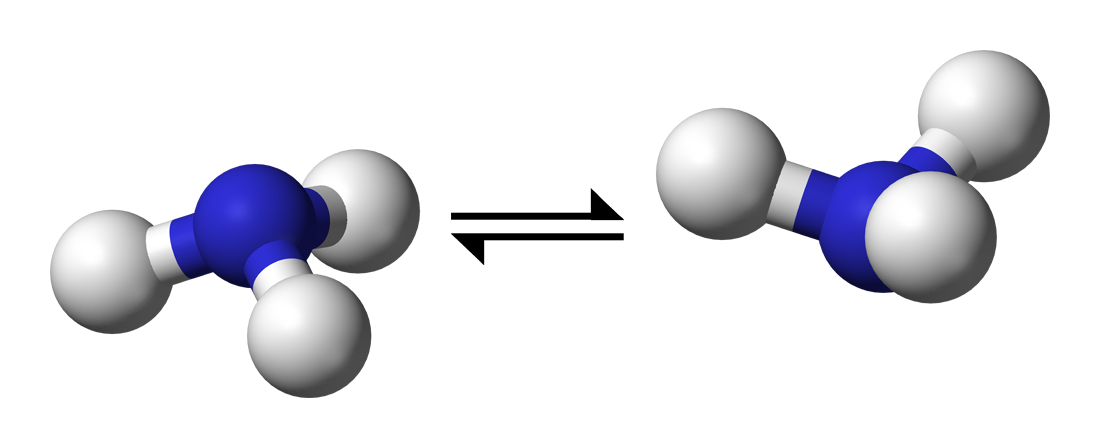
\includegraphics[scale=0.3]{img/Nitrogen-inversion-3D-balls (1).png}
    \caption{Stickstoff- (oder Schirm-) Inversion in Ammoniak. \refimgsource{Wikimedia}{https://commons.wikimedia.org/wiki/File:Nitrogen-inversion-3D-balls.png}{18.01.2022}{public domain}}
    \label{fig:my_label}
\end{figure}

\begin{fquestion}{Wie ist die Formel für gemischte Zustände mit den dazugehörigen Energien?}
    Die Formel für den gemischten Zustand ist hier
    \[\ket{\Psi(t)} = \sum_n c_n \ket{\psi_n} \e^{-\frac{\i}{\hbar} E_n t} = c_1 \ket{1} \e^{-\frac{\i}{\hbar} E_1 t} + c_2 \ket{2} \e^{-\frac{\i}{\hbar} E_2 t}\]
    wobei $\ket{1}$ und $\ket{2}$ jeweils die beiden Symmetriezustände (Stickstoff ober- oder unterhalb der Wasserstoffebene beschreiben).
    Der Hamiltonian des Systems ist allgemein
    \[H = \begin{pmatrix} E_0 & -A \\ -A & E_0 \end{pmatrix}\]
    mit der Grundenergie der beiden Symmetriezustände $E_0$ und der Energie aus dem Überlappintegral $A = \braket{1 | H}{2}$.
    Die Eigenenergien sind
    \[E_\pm = E_0 \pm A.\]
\end{fquestion}

% \begin{question}{Zeichnung gekreuzte Zustände ohne E-Feld? (Zeichnung Amoniak Molekül)}
%     Mittelpunkt der linearen Kreuzung ???
%     Wo liegen sie mit Feld? 
%     auf y-Achse im Minimum der ALC ???
%     Skizze mit den Zustandsenergien als Hyperbeln ???
%     Landau-Zehner-Wahrscheinlichkeit ???
% \end{question}

\begin{fquestion}{Welchen Einfluss hat das Elektrische Feld?}
    Das elektrische Feld führt aufgrund des Dipolmomentes $p$ in Symmetriezustände zu einer Unterscheidung beiden, wobei \(E_1 = E_0 + p \mathcal{E}\) und \(E_1 = E_0 - p \mathcal{E}\).
    Damit ändern sich die Eigenenergien zu
    \[E_\pm = E_0 \pm \sqrt{A^2 + p^2 \mathcal{E}^2}.\]
\end{fquestion}

\begin{fquestion}{Wieso spielt das elektrische Feld eine Rolle?}
    Das elektrische Feld ermöglicht ein kontrolliertes Anfahren des Level-Crossings (siehe Maser).
\end{fquestion}

\begin{figure}[H]
    \centering
    % \includesvg[scale=0.4]{img/Stern-Gerlach_experiment_svg.svg}
    \includegraphics[width=0.9\linewidth]{img/Stern-Gerlach_experiment_svg.png}
    \caption{Stern–Gerlach experiment: Silver atoms travelling through an inhomogeneous magnetic field, and being deflected up or down depending on their spin; (1) furnace, (2) beam of silver atoms, (3) inhomogeneous magnetic field, (4) classically expected result, (5) observed result. \refimgsource{Wikimedia}{https://commons.wikimedia.org/wiki/File:Stern-Gerlach_experiment_svg.svg}{18.01.2022}{Creative Commons Attribution-Share Alike 4.0 International}}
    \label{fig:zustandsmischung:stern-gerlach}
\end{figure}

\begin{fquestion}{Wie kann man die Mischung sichtbar machen?}
    Die Mischung kann mit einem Stern-Gerlach Apparat sichtbar gemacht werden, siehe \autoref{fig:zustandsmischung:stern-gerlach}. 
    Durch ein inhomogenes Feld quer zur Strahlachse erfolgt eine Auftrennung der Zustände.
    Durch ein langsames Absenken des Feldes, wird verhindert, dass die Zustände direkt wieder durch Tunneln mischen.
\end{fquestion}

\begin{fquestion}{Wie kann man das experimentell überprüfen?}
    Durch einen Maser.
    Für NH${}_3$ ist $\omega = \SI{24}{GHz}$.
\end{fquestion}

\begin{fquestion}{Wie ist der Mischungswinkel?}
    Es ist $\theta_m = \SI{45}{\degree}$.
\end{fquestion}

\subsection{Avoided Level Crossing (ALC)}

\begin{figure}[H]
    \centering
    \begin{tikzpicture}[scale=4,cap=round]
        
        \coordinate (A) at (0,0);
        \coordinate (B) at (1.5,1);
        \coordinate (C) at (0,1);
        \coordinate (D) at (1.5,0);
        \coordinate (M) at (0.75,0.5);
        
        \coordinate (CO) at (-0.25, -0.15);
        \coordinate (CT) at (-0.25, 1.25);
        \coordinate (CR) at (1.75, -0.15);
        \coordinate (CM) at (0.75, -0.15);
        
        \draw[color=blue, thick] (A) .. controls (M) ..  (D);
        \draw[color=blue, thick] (B) .. controls (M) ..  (C);
        \draw[dashed] (A) to (B);
        \draw[dashed] (C) to (D);
        
        \node[anchor=east] at (A) {$\ket{1}$};
        \node[anchor=west] at (B) {$\ket{1'}$};
        \node[anchor=east] at (C) {$\ket{2}$};
        \node[anchor=west] at (D) {$\ket{2'}$};
        
        
        \node[anchor=south,text=blue] at ($(M)+(0,0.2)$) {$\ket{\phi_2}$};
        \node[anchor=north,text=blue] at ($(M)-(0,0.2)$) {$\ket{\phi_1}$};
        
        \draw[color=black, -{Stealth[length=3mm,width=2mm]}] (CO) to (CT);
        \draw[color=black, -{Stealth[length=3mm,width=2mm]}] (CO) to (CR);
        
        \node[anchor=south] at (CT) {$V(z)$};
        \node[anchor=west] at (CR) {$z$};
        
        \draw[color=black] ($(CM)+(0,-0.025)$) to ($(CM)+(0,0.025)$);
        \node[anchor=north west] at (CM) {$z_c$};
        
    \end{tikzpicture}
    \caption{Skizze eines Avoided Crossing. Im Graph sind die Energien eines Systems in Abhängigkeit einen Parameters $z$ dargestellt. Die gestrichelte Linie entspricht dem diabatischen (schnellen) Übergang, bei dem ein Crossing der Eigenzustände $\ket{1}$ und $\ket{2}$ bei $z_c$ stattfindet, die durchgezogenen Linien entsprechen dem adiabatischen (langsamen) Übergang (den Eigenwerten $\ket{\phi_1}$ und $\ket{\phi_2}$ des Hamiltonians).}
\end{figure}

\begin{fquestion}{Was ist Avoided Level Crossing?}
    Von einem Avoided Level Crossing spricht man, wenn die Energieeigenwerte eines Systems von einem kontinuierlichen Parameter (etwa der Zeit $t$ oder einem äußeren Feld $\mathcal{E}$) abhängen und sich in Abhängigkeit dessen nicht berühren.
    Beim Durchfahren eines Level Crossing kann ein Zustand in einen anderen übergehen (natürlich auch schon vorher, aber hier werden sich die Zustände immer ``ähnlicher'').
\end{fquestion}

\begin{fquestion}{Was ist das Landau-Zener Modell?}
    Im Landau-Zener Modell werden folgende Annahmen getroffen:
    \begin{enumerate}
        \item Der Störparameter ist eine bekannte, lineare Funktion in der Zeit (etwa ein linear verfahrendes E-Feld).
        \item Die Energielücke zwischen den diabatischen Zuständen variiert linear in der Zeit
        \item Die Kopplung im diabatischen Hamiltonian ist zeitunabhängig
    \end{enumerate}
    Die Übergangswahrscheinlichkeit ist dann
    \[ P_{mn} = 1 - \exp \left( -\frac{ \pi \Delta_{m n}^2}{2\hbar g \mu_B |m - n| \mu_0 \dd E / \dd t} \right) = 1 - \exp(\Gamma_{mn} \dd t). \]
\end{fquestion}

\begin{fquestion}{Was bedeutet es sich diabatisch bzw. adiabatisch einen Level-Crossing anzunähern?}
    Bei der diabatischen Annäherung wird das Level-Crossing schnell ($\dd t$ sehr klein) angefahren, ein Zustandsübergang findet also eher nicht statt. 
    Die adiabatischen Annäherung findet langsam ($\dd t$ sehr groß) statt und entsprechend folgen die Zustände den Eigenzustände des Hamiltonian.
    \begin{center}
        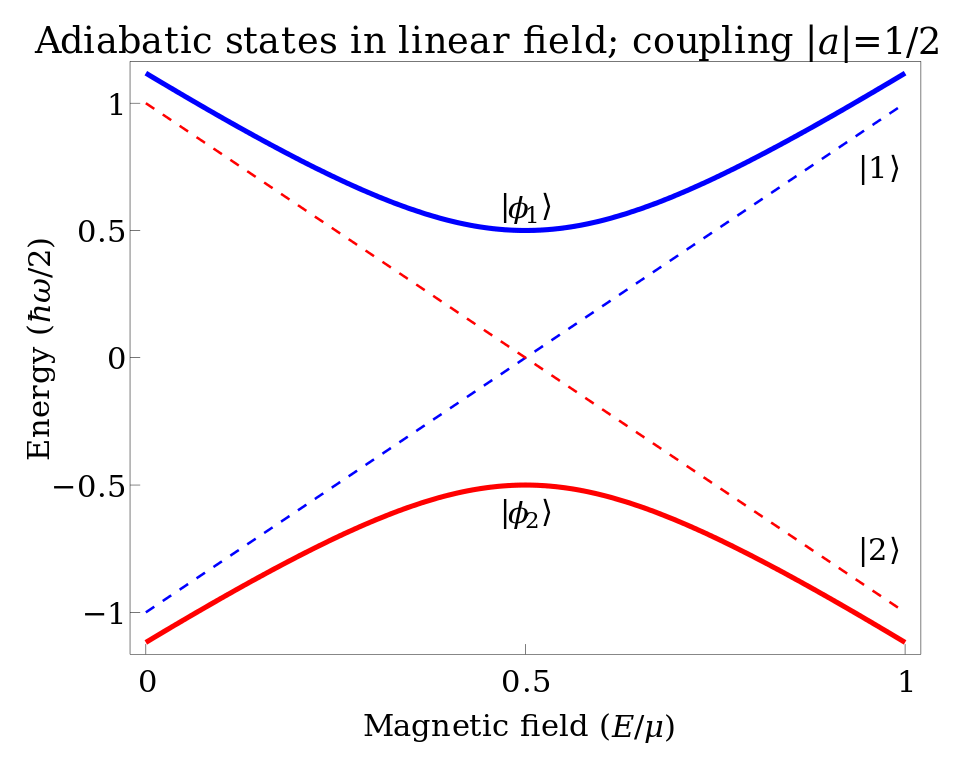
\includegraphics[scale=0.2]{img/Avoided_crossing_in_linear_field.svg.png}
    \end{center}
    Skizze zu einem Avoided Level Crossing eines Zwei-Niveau-Systems im magnetischen Feld. \refimgsource{Wikimedia}{https://commons.wikimedia.org/wiki/File:Avoided_crossing_in_linear_field.svg}{18.01.2022}{Creative Commons CC0 1.0 Universal Public Domain Dedication} 
\end{fquestion}

% \begin{question}{Was passiert jetzt wenn ich so einen strahl aus dem Feld herausbringe und mir den zeitlichen Verlauf der Mischungszustände und symmetriezustände anschaue?}
%     Da wusste ich nicht worauf sie hinaus wollten, sie wollten etwas über den mischungswinkel hören ???
    
%     Als Nächstes kam eine Frage, mit der ich erst nichts anzufangen wusste. Es ging so ungefähr wie: Was benötigt man denn, damit diese Spinzustände mischen, da Spinzustände ja eigentlich sonst Eigenzustände sind. Dann haben sie wieder etwas von energetisch und symmetrien gesprochen. Das waren wieder Signalworte. Kurz Hamilton skizziert wobei die planare Anisotropie nicht null sein darf, also die planare Anisotropie ist der "Wechselwirkungsterm" der dann zur Mischung führt. Damit waren sie zufrieden.
%     Und sie fragten noch, wie man diese Mischung denn dann beeinflussen kann. Dabei wollten sie darauf hinaus, dass man mithilfe von Magnetfeldern in der x-y-Ebene genau diese planare Anisotropie beinflusst.
% \end{question}

\subsection{Maser}

\begin{fquestion}{Wie funktioniert er?}
    % Skizze von Boltzmann-Verteilung N(E) ???
    % Besetzungsinversion für stimulierte Emission (siehe Laser: Pumpen), hier über Strahltrennung ???
    % Strahltrennung?
    % zu Beginn hohes Feld, damit Symmetrie den Energiezuständen entspricht ??? 
    % Strahlen mit einem inhomogenen eletrischen Feld trennen (ausnutzen, dass elektrische Dipolmomente der Symmetriezustände verschieden ausgerichtet sind -> Kraft von E-Feld unterschiedlich)
    % langsam elektrisches Feld senken, um wieder einen perfekt gemischten Zustand zu bekommen ??? 
    % im Hohlraumresonator und mit stimulierter Emission erhält man kohärentes Laserlicht (Mikrowellen, da maser, also meV)
    
    Der Aufbau besteht aus einem Strahltrenner mit inhomogenem elektrischen Feld $\epsilon_\text{inh.}$ und einer Kavität mit oszillierendem Feld $\epsilon_\text{ac}(t)$.
    \\
    Das Feld des Strahlteilers muss inhomogen sein, weil sich die Dipolmomente in einem homogenen Feld lediglich parallel zum Feld ausrichten.
    Damit eine Kraft entsteht, darf der Gradient des Felds also nicht verschwinden.
    In Abbildung \ref{fig:AmmoniakALC} befindet sich das System nun ganz rechts, wobei hier für die Eigenzustände näherungsweise $\ket{\psi_+}\approx \ket{1}$ und $\ket{\psi_-}\approx \ket{2}$ gilt (entspricht Mischungswinkel von $\theta\approx \SI{90}{\degree}$).
    Bei adiabatischer Absenkung des Feldes ``wandern'' die Zustände dann entlang der blauen Kurven, die den Eigenenergien 
    $$E_\pm = E_0 \pm \sqrt{A^2 + (\Vec{d}\cdot\Vec{\epsilon})^2}$$
    entsprechen.
    Für $\epsilon\approx 0$ befindet sich ein Großteil der Moleküle der beiden Strahle dann in einem der Eigenzustände wieder.
    \\
    Interessant ist hierbei der Anteil mit einer Eigenenergie von $E_0 + A$.
    Dieser wird nun in die Kavität geleitet.
    Mit etwas Mathematik kann man zeigen, dass die Periodendauer der angeregten Oszillation $T=\frac{\pi\hbar}{2|\Vec{d}||\Vec{\epsilon}_0|}$ entspricht.
    Die Moleküle sollten bei einer Geschwindigkeit $v$ und einer Länge der Kavität $L$ also gerade die Zeit $T$ in dieser verbringen, um (nahezu) vollständig in den niederenergetischen Eigenzustand $E_-$ überführt zu werden.
    Die Frequenz der dabei abgestrahlten Photonen ist $\omega = 2 A$.
\end{fquestion}

% NH3-Maser
\begin{figure}[!ht]
    \centering
    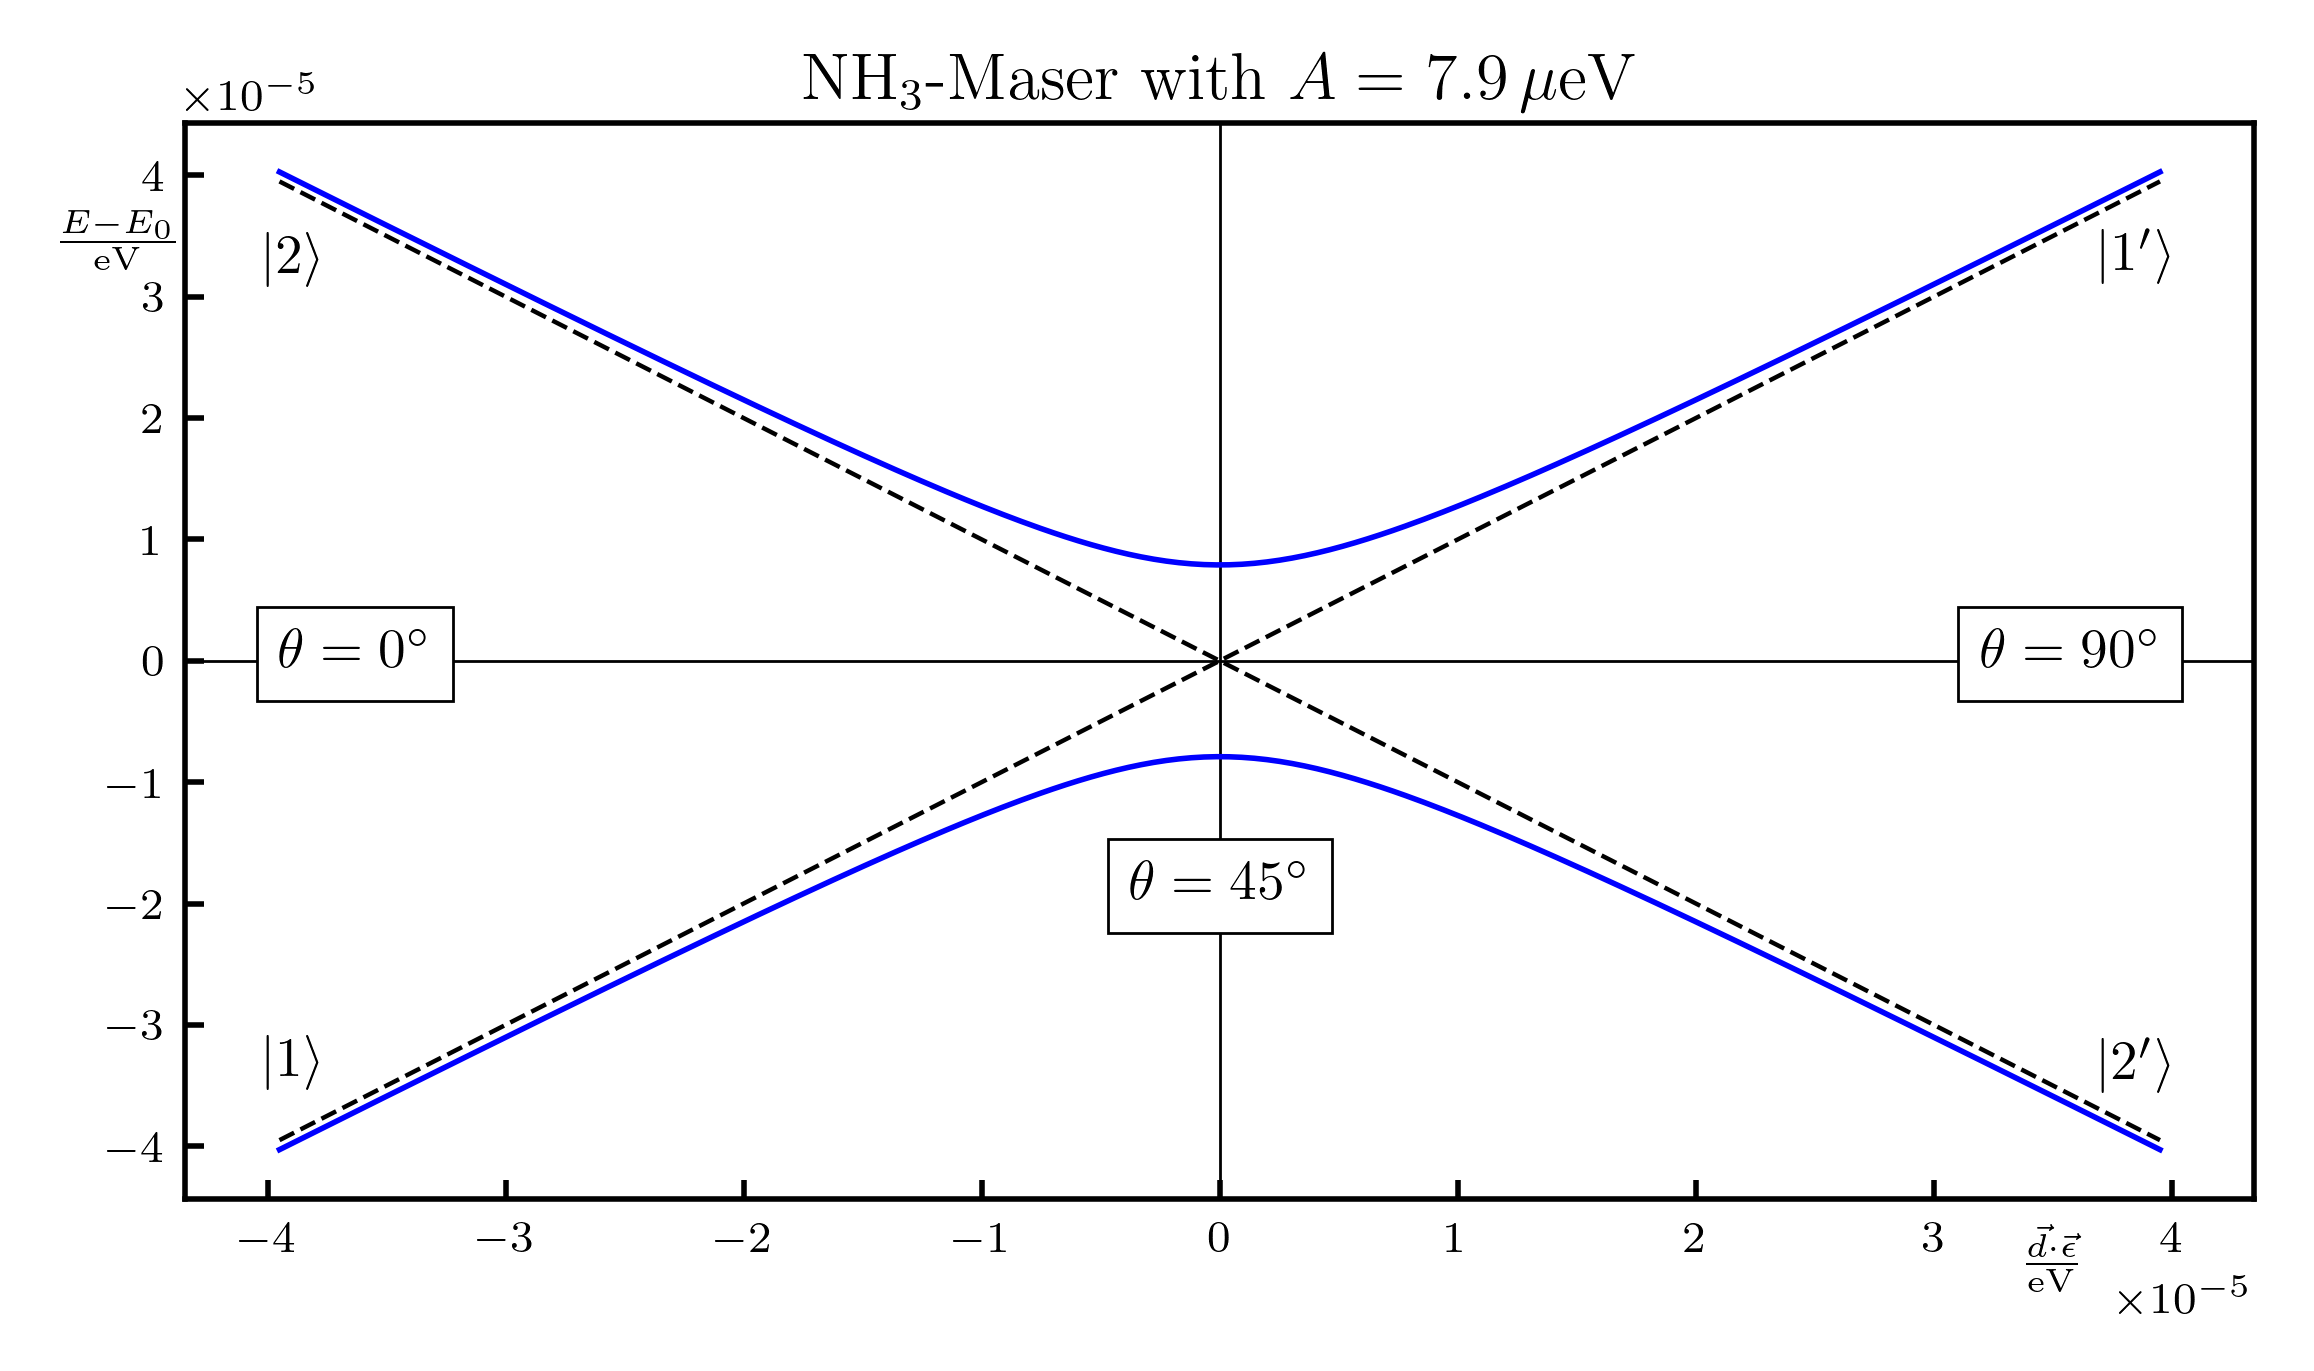
\includegraphics{img/AmmoniakALC.png}
    \caption{Vermiedene Kreuzungen für Ammoniak mit Dipolmoment $\Vec{d}$ in einem elektrischen Feld $\Vec{\epsilon}$.
    Der jeweilige Mischungswinkel ist als $\theta$ vermerkt.}
    \label{fig:AmmoniakALC}
\end{figure}

\begin{fquestion}{Warum inhomogenes Feld?}
    Im homogenen Feld nur Ausrichtung der Dipolmomente, aber keine Kraft.
\end{fquestion}

\begin{fquestion}{Warum sollte man das elektrische Feld langsam ändern?}
    Es tritt ein Landau-Zener Übergang mit der Tunnelwahrscheinlichkeit 
    \[P = e^{-\gamma}, \quad \gamma = \frac{|H_{12}|^2}{\dd E/\dd t}\]
    auf.
    Dieser ist abhängig von der Energie-Lücke, aber auch von der Energie-Änderungsrate.
\end{fquestion}

% \begin{question}{Wieso kommt es zum Aufspalten der Zustände?}
% \end{question}

% \begin{question}{Wie ist die Zustandsverteilung im oszillierenden Feld?}

% \end{question}

% \begin{question}{Die strahlenden Übergänge starten durch spontane Emissionen, dadurch werden wie bei laser weitere angeregt. Warum muss ich bei kleinen E-Feldern aufpassen?}
%     Langsam ändern lassen, damit nicht tunneln
% \end{question}

% \begin{question}{Energetische Betrachtung?}
%     Schema der vermiedenen Niveaukreuzungen
% \end{question}


\begin{fquestion}{Was sind andere Anwendungen des Masers?}
    Ein weiterer Maser ist der Wasserstoffmaser, bei dem die Hyperfeinstrukturaufspaltung von Wasserstoff im Grunzustand mit einer Frequenz 
    $$E_{\mathrm{HFS}} = \SI{1420405751.767}{Hz}$$
    genutzt wird.
    Zunächst werden die Atome im Zustand $F = 1$ (parallele Ausrichtung von Kern und Elektron) von denen im $F=0$ selektiert (etwa durch Zeeman-Aufspaltung im starken Magnetfeld).
    Eingeleitet in eine Kavität (mit Teflon beschichtet, damit die Wasserstoffmoleküle nicht binden können), herrscht dort eine Besetzungsinversion zwischen dem $F=1$ und $F=0$-Niveaus, wodurch eine stimulierte Emission mit genau der Hyperfeinstrukturaufspaltung beobachtet werden kann.
    
    Diese Frequenz ist so genau ($\mathcal{O}(10^{-12})$), dass sie zur präzisen Zeitmessung genutzt werden kann.
\end{fquestion}

% \subsection[${\text{Mn}}_{12}$-Acetat]{$\mathbf{\textbf{Mn}_{12}}$-Acetat}
% \subsection{$\mathbf{\textbf{Mn}_{12}}$-Acetat}
\subsection{Magnetische Moleküle}

\begin{figure}[htb]
    \centering
    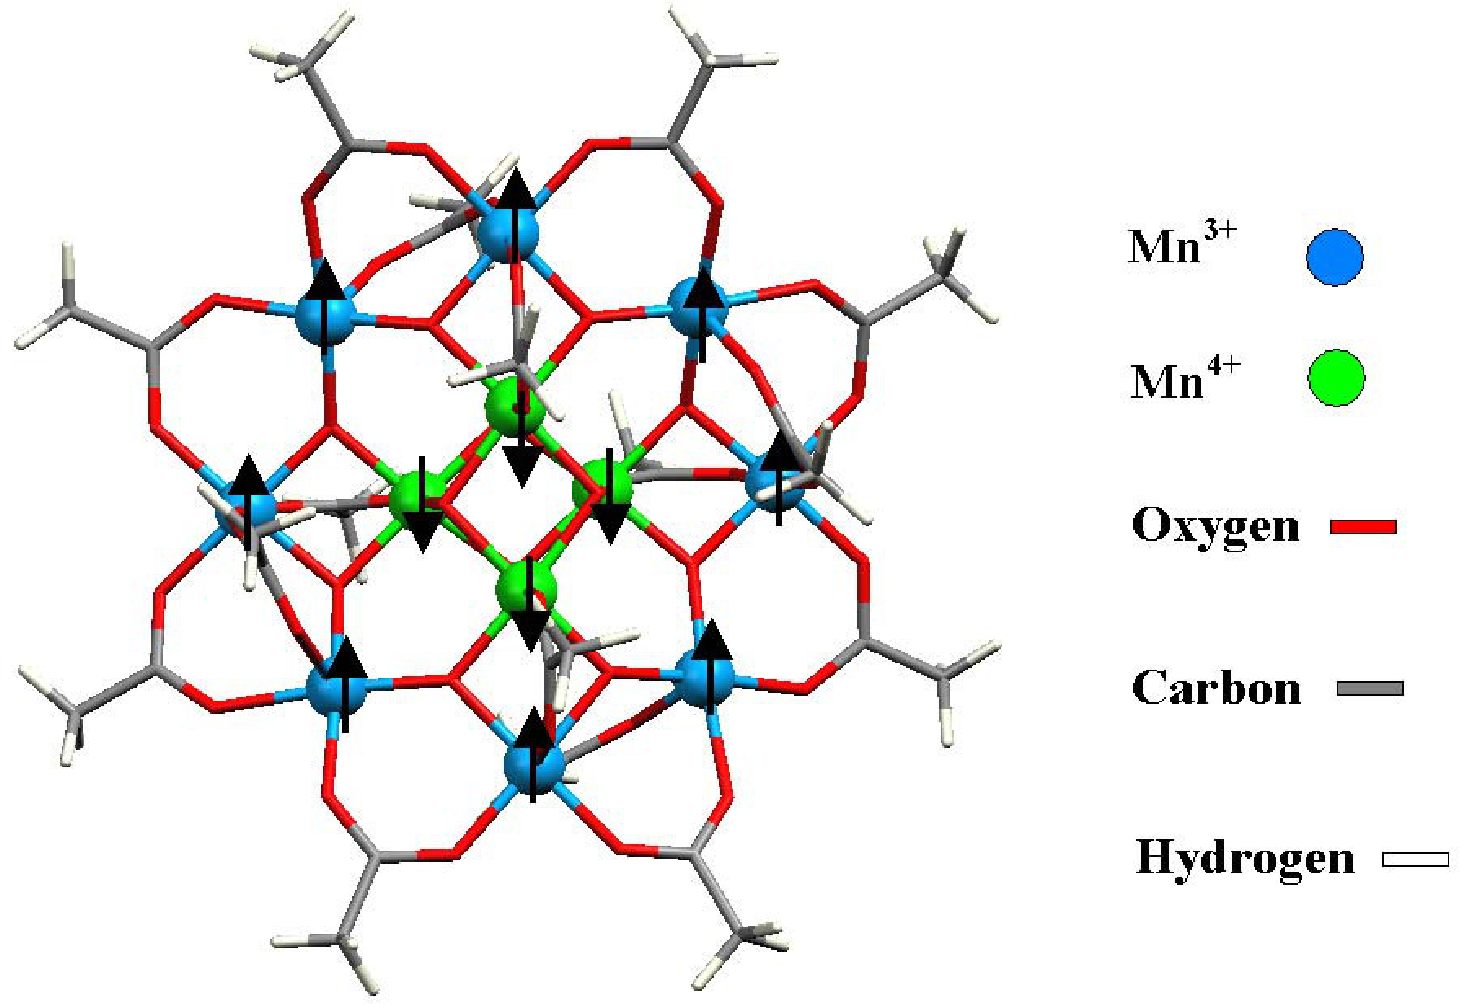
\includegraphics[width=0.5\linewidth]{img/17-Figure1.1-1.png}
    \caption{Skizze des $\text{Mn}_{12}$-Acetats. Dabei hat $\text{Mn}^{\text{III}}$ einen Spin von $s=2$ und $\text{Mn}^{\text{IV}}$ einen Spin von $s=3/2$.}
    \label{fig:mn12acetat}
\end{figure}

\begin{figure}
    \centering
    \begin{subfigure}{0.77\linewidth}
        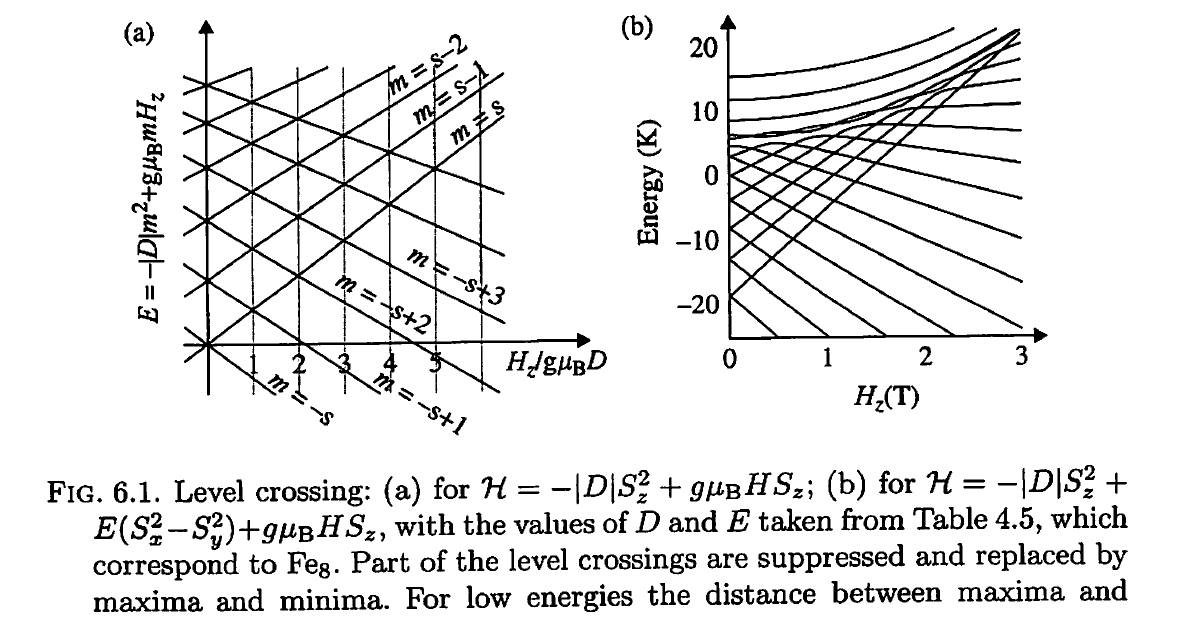
\includegraphics[width=\linewidth]{img/mn12_level_crossing.png}
    \end{subfigure}
    \begin{subfigure}{0.21\linewidth}
        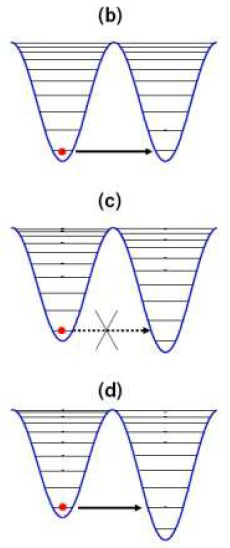
\includegraphics[width=\linewidth]{img/mn12_tunneling.png}
    \end{subfigure}
    \begin{subfigure}{0.9\linewidth}
        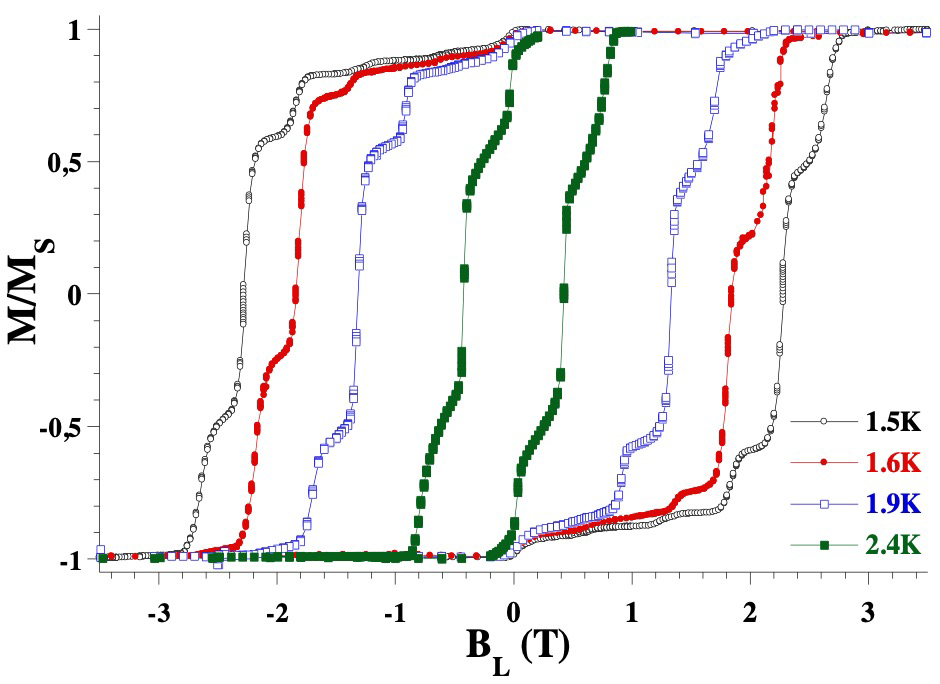
\includegraphics[width=\linewidth]{img/mn12_hysteresis.png}
    \end{subfigure}
    \caption{Übersicht über Energieniveauverlauf, Tunnelvorgang und Hysterekurve beim $\text{Mn}_{12}$-Acetat. Aus der Vorlesung entnommen.}
    \label{fig:mn12vis}
\end{figure}

\begin{fquestion}{Was misst man beim $\text{Mn}_{12}$-Acetat?}
    Beim magnetischen Molekül $\text{Mn}_{12}$-Acetat ($S = 10$) (alternativ auch beispielsweise beim $\text{Ni}$-Quadrumer oder beim $\text{V}_{15}$ ($S = 1/2$), $\text{Ni}_{12}$ ($S = 12$) oder $\text{Fe}_8$ ($S = 10$)) bilden sich entsprechend der Ausrichtung des Spins $m_s$ diskrete Magnetisierungen.
    Ohne externes Magnetfeld bilden diese unter dem Hamiltonian $H = -D S_z^2 + E (S_x^2 - S_y^2)$ zwei Parabeln mit entartetem Grundniveau $\ket{m_s = 10}$ und $\ket{m_s = -10}$.
    Wird ein externes Magnetfeld angelegt, wird durch $H = g \mu_B \mu_0 S H_{\text{ext}}$ die Entartung aufgehoben und bei bestimmten externen Magnetfeldern kreuzen sich die ursprünglichen Eigenzustände.
    
    An diesem Beispiel kann das Avoided-Level-Crossing sehr schön experimentell nachvollzogen werden, für Grafiken siehe \autoref{fig:mn12vis}.
\end{fquestion}

\subsection{Neutrinooszillation}

\begin{figure}[!ht]
    \centering
    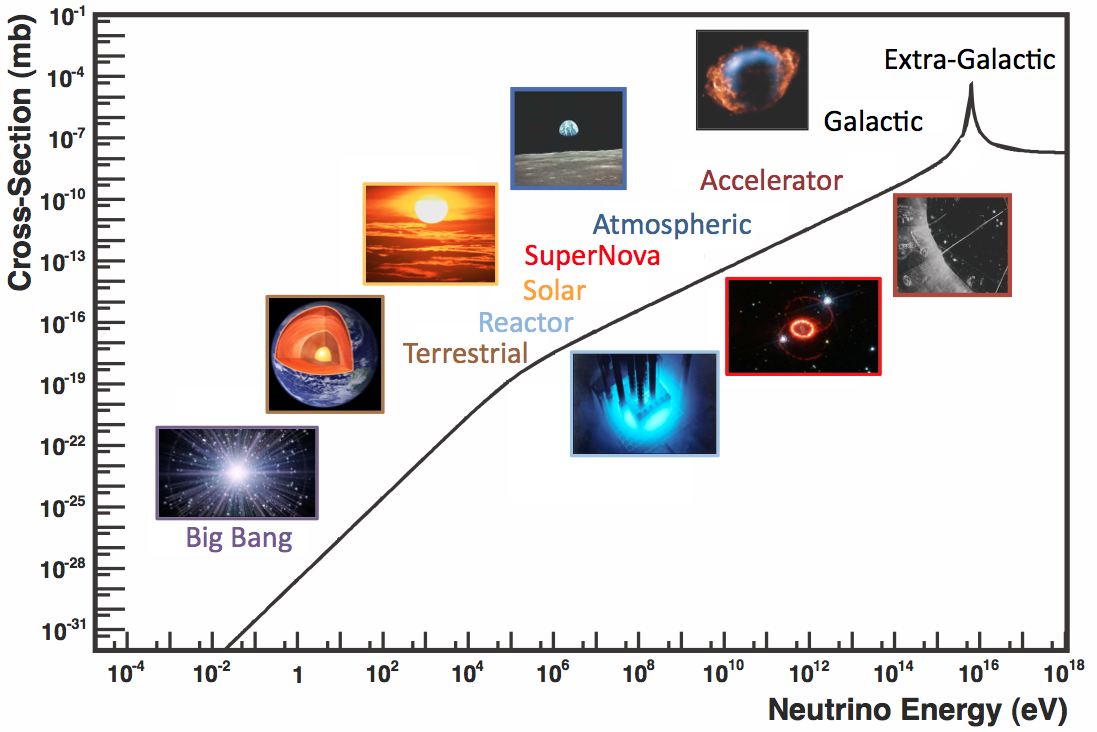
\includegraphics[width=\linewidth]{img/Neutrino_Wirkungswuerschnitt.png}
    \caption{Wirkungsquerschnitt von Neutrinos in Abhängigkeit der Energie mit $W^\pm$ Resonanz bei $\SI{10E16}{\electronvolt}$. Eine mögliche Quelle der Neutrinos mit entsprechenden Energien ist vermekt.
    \refimgsource{From eV to EeV: Neutrino Cross-Sections Across Energy Scales}{https://arxiv.org/pdf/1305.7513.pdf}{18.01.2022}{keine}}
\end{figure}

\begin{fquestion}{Wieso gibt es bei den Neutrinos Zustandsmischungen?}
    Entsprechend der PMNS (Pontecorvo–Maki–Nakagawa–Sakata) Matrix
    \[U_{\mathrm{PMNS}} \approx \begin{pmatrix}
        0.8 & 0.6 & 0.1 \\
        0.4 & 0.5 & 0.7 \\
        0.4 & 0.5 & 0.7 
    \end{pmatrix}\]
    mit den Mischwinkeln $\theta_{12} = \SI{33}{\degree}$, $\theta_{23} = \SI{49}{\degree}$ und $\theta_{13} = \SI{9}{\degree}$ sind die Flavoureigenzustände aus Masseneigenzuständen ${\nu_{\mathrm{Flavour}} = U_{\mathrm{PMNS}} \nu_{\mathrm{Masse}}}$ zusammengesetzt. 
    Letztere breiten sich mit unterschiedlichen Frequenzen entsprechend der Energien aus, wodurch es zu Intereferenzen kommt.
    In der Flavourprojektion zeigen sich diese durch Oszillationen zwischen verschiedenen Flavourzuständen.
\end{fquestion}

\begin{fquestion}{Wie kommt die Oszillation aus der Zeitentwicklung zustande?}
    Die Eigenzustände entwickeln sich gemäß $\ket{\nu_{1,2}(t)} = \e^{-\i E_{1,2}t} \ket{\nu_{1,2}},$ wobei die Eigenenergien durch 
    $$E_{1,2} = \sqrt{m_{1,2}^2 + p^2} \approx p + \frac{m_{1,2}^2}{2p} $$
    gegeben sind.
    Hierbei ist insbesondere die Energiedifferenz relevant, welche über $\Delta m_{12}^2 = m_2^2 - m_1^2 \approx \SI{7.5e-5}{eV^2}$ gegeben ist.
    Da im Vakuum $\ket{\nu_e} = \cos\theta_{12}\ket{\nu_1} + \sin\theta_{12}\ket{\nu_2}$ ist, folgt die Zeitentwicklung entsprechend
    $$\ket{\nu(t)} = \e^{-\i E_{1}t} \cos\theta_{12}\ket{\nu_1} + \e^{-\i E_{2}t} \sin\theta_{12}\ket{\nu_2}.$$
    % psi(t) = c1(t) |1> + c2(t) |2> und wie c1 und c2 aussehen und warum (also kurz für Eigenzustände Zeitentwicklung benannt)
    % Koeffizienten über Anfangsbedingung
    Die Neutrinos bewegen sich beinahe mit Lichtgeschwindigkeit, also  $v \sim c$.
    Damit können wir anstatt Zeit auch Entfernung betrachten, also $ t\sim x$ (z.B. bei atmosphärischen Neutrinos gut zu erkennen). 
    Die Überlebenswahrscheinlichkeit ist dann gegeben durch
    $$P_{ee}(x) = |\braket{\nu_e }{ \nu (x)}|^2 = \left\vert \e^{-\i \frac{m_1^2}{2E}x} \cos^2\theta_{12} + \e^{-\i \frac{m_2^2}{2E}x} \sin^2\theta_{12} \right\vert^2.$$
    Eine ausführliche Rechnung liefert dann
    $$P_{ee}(x) = 1 - \sin^2 2\theta_{12} \sin^2\left( \frac{\Delta m_{12}^2}{4E} x \right).$$
\end{fquestion}

\begin{fquestion}{Was ist der Störparameter bei der Neutrinooszillation?}
    Die Elektronendichte (bei $\nu_e$-Oszillation) des umliegenden Mediums.
\end{fquestion}

\begin{fquestion}{ALC in der Sonne, was passiert da genau?}
    % Elektronneutrino zu Myonneutrino  (auch tau)
    Durch die Elektronendichte $n_e(r) = n_0\e^{-r/r_0}$ gibt es in der Sonne einen zusätzlichen Term, der zur Masse der Elektronneutrinos beiträgt $$\Delta m_N^2(r) = 2E\sqrt{2}G_F n_e(r).$$
    Im Vakuum gilt
    $$\begin{pmatrix}
     | \nu_e \rangle \\  | \nu_\mu  \rangle
    \end{pmatrix} = \begin{pmatrix}
    \cos\theta & \sin\theta \\ -\sin\theta & \cos\theta
    \end{pmatrix} \begin{pmatrix}
     | \nu_1 \rangle \\  | \nu_2 \rangle
    \end{pmatrix},$$
    wobei durch die Materie der Mischungswinkel verändert wird.
    Die Erwartungswerte der Massen der Flavour-Neutrinos sind hier
    $$m_{\nu_e}^2 = \langle \nu_e | \hat{m}^2 | \nu_e \rangle = m_{\nu_1}^2 \cos^2\theta + m_{\nu_2}^2 \sin^2\theta = \Delta m_{12}^2 \sin^2\theta + m_{\nu_1}^2,$$
    $$m_{\nu_\mu}^2 = \langle \nu_\mu | \hat{m}^2 | \nu_\mu \rangle = m_{\nu_1}^2 \sin^2\theta + m_{\nu_2}^2 \cos^2\theta = \Delta m_{12}^2 \cos^2\theta + m_{\nu_1}^2.$$
    Wegen des MSW-Effekt (Michejew-Smirnow-Wolfenstein) ändern sich die Massen-Eigenzustände zu
   $$\tilde{m}^2_{\nu_1,\nu_2} - m_{\nu_1}^2 = \frac{1}{2}\left( \Delta m_{12}^2 + \Delta m_N^2(r) \pm \Delta \tilde{m}^2(r) \right),$$
    wobei die Massen-Lücke durch
    $$\Delta \tilde{m}^2(r) = \sqrt{\left( \Delta m_{12}^2 \cos 2\theta_{12} - \Delta m_N^2 (r) \right)^2 + \left( \Delta m_{12}^2 \sin 2\theta_{12} \right)^2 }$$
    Abbildung \ref{fig:solar neutrino msw theta 34} zeigt die Entwicklung der Zustände in der Sonne.
\end{fquestion}

\begin{figure}[!ht]
    \centering
    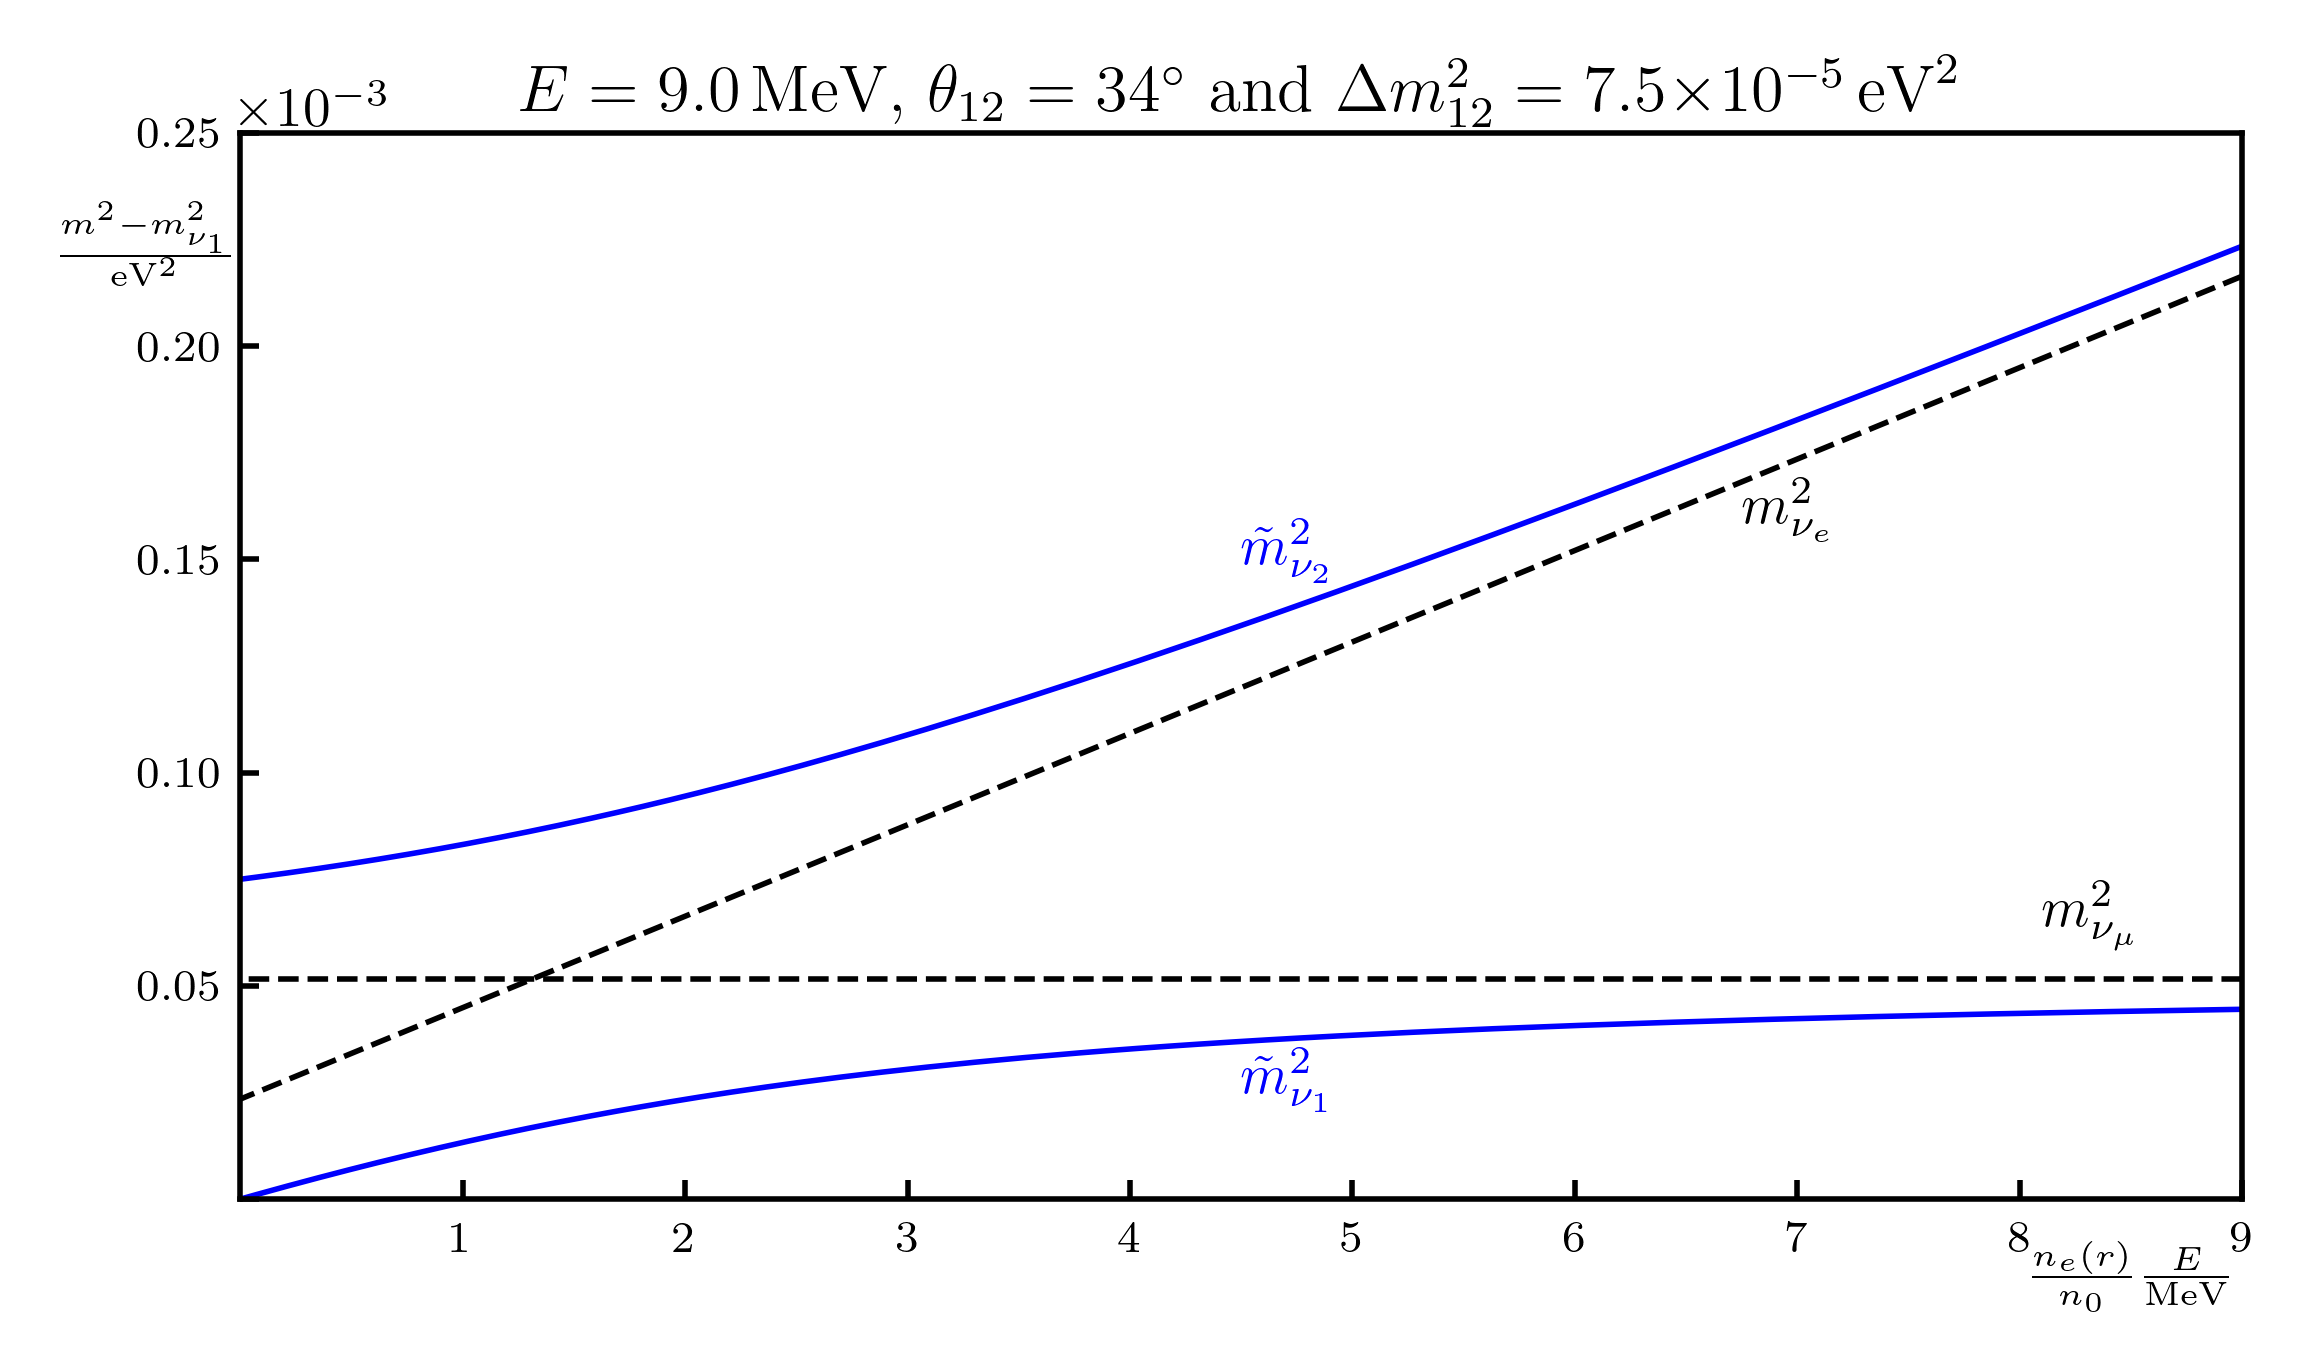
\includegraphics{img/SolarNeutrinoALC_theta34v3.png}
    \caption{Visualisierung der Entwicklung der Massen-Eigenzustände $ | \tilde{\nu}_{1,2} \rangle$ in der Sonne.
    Die $x$-Achse entspricht der Elektronendichte, das Sonnenzentrum ist also rechts, das (fast-)Vakuum links.}
    \label{fig:solar neutrino msw theta 34}
\end{figure}

\begin{fquestion}{Was sind jeweils die geraden Linien im Diagramm}
    Die Erwartungswerte der Massen der Flavour-Eigenzustände.
    Der für das Elektron-Neutrino hängt von der Elektronendichte ab.
    Der Kreuzungspunkt wandert für höhere Energien nach links, also zum Sonnenrand hin, weil der Anstieg der $\nu_e$-Geraden größer wird.
\end{fquestion}


\begin{fquestion}{Was ist der MSW-Effekt?}
    Beschreibt den Einfluss von Materie auf die Neutrino-Oszillationen. 
    Durch die Elektronendichte erhält der Elektron-Neutrino Zustand eine zusätzliche Masse über die Wechselwirkung mit $W^\pm$.
    Das Feynman-Diagramm für Geladene Ströme (also über $W^\pm$) ist für Myon- und Tau-Neutrinos nicht möglich.
\end{fquestion}

\begin{fquestion}{Was ist die Ursache dafür?}
    Aufgrund der Erhaltung der Flavour-Zahl ist das Feynman-Diagramm für die Streuung der anderen Neutrinos an Elektronen über $W^\pm$ verboten.
\end{fquestion}

\begin{fquestion}{Warum gibt es denn nur Elektronen in der Sonne?}
    Energie der solaren Neutrinos liegt in der Größenordnung  $1\dots 10\,$MeV, also deutlich unterhalb der Masse von Myonen oder Taus.
\end{fquestion}

\begin{fquestion}{Wie werden Neutrinos in der Sonne produziert?}
    Die dominierende Reaktionsgleichung lautet
    \[p + p \rightarrow d + e^+ + \nu_e.\]
    Es verschmelzen zwei Protonen zu einem Deuterium-Kern, einem Positron und einem $e$-Neutrino.
    Das entsprechend Feynman-Diagramm ist in \autoref{fig:neutrino_prod_sonne}.

    Die weiteren Prozesse sind die folgenden:
    
    \begin{center}
        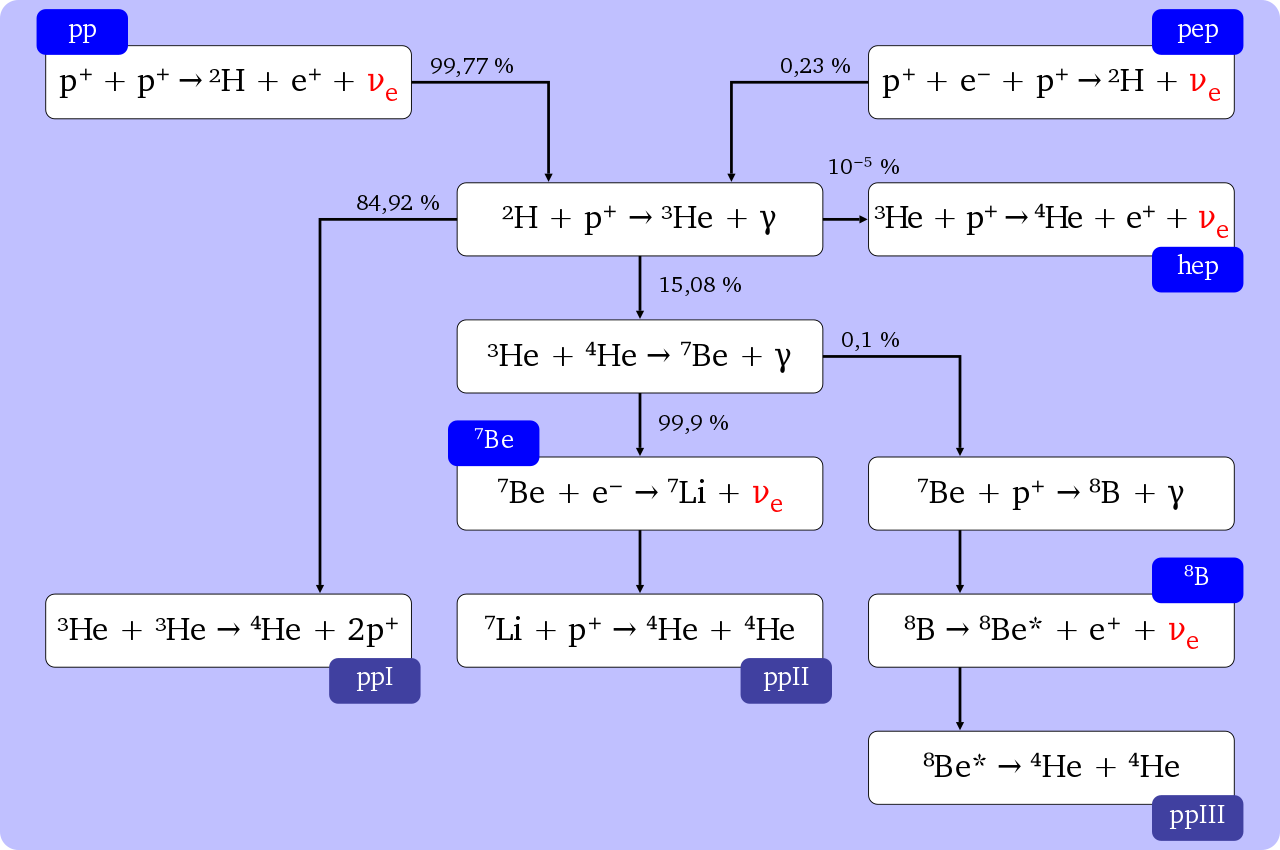
\includegraphics[width=.9\linewidth]{img/1280px-Proton_proton_cycle.svg.png}
    \end{center}
    
    \refimgsource{Wikimedia}{https://upload.wikimedia.org/wikipedia/commons/thumb/a/ac/Proton_proton_cycle.svg/1280px-Proton_proton_cycle.svg.png}{20.01.2022}{Creative Commons Attribution-Share Alike 2.5 Generic}

\end{fquestion}

\begin{figure}[!ht]
    \centering
    % 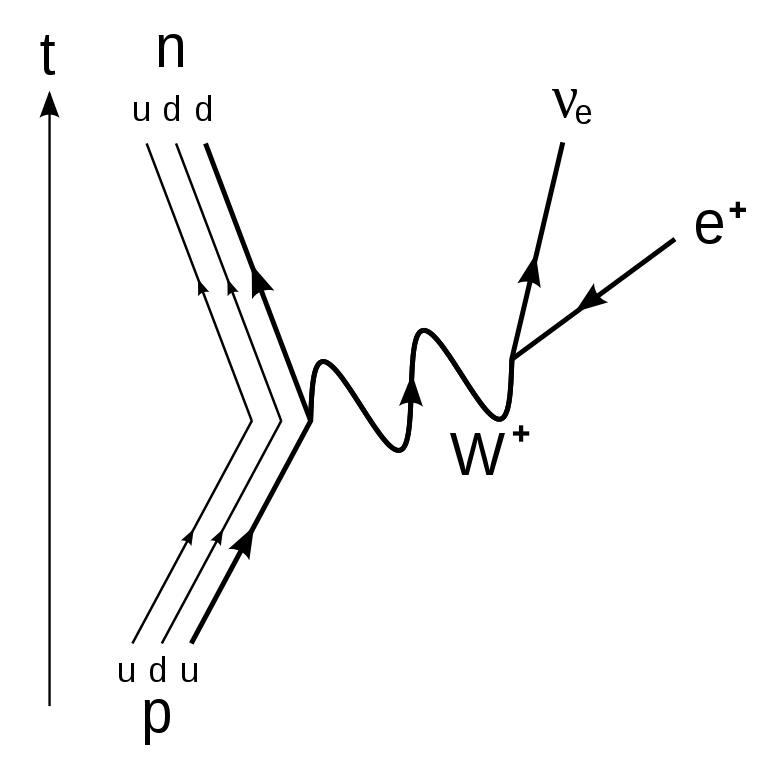
\includegraphics[scale=0.3]{img/768px-Electron_Capture_Decay.svg.png}
\begin{tikzpicture}[x=20mm, y=20mm]
\begin{feynman}[]
    \vertex (i1) {\(u\vphantom{d}\)};
    \vertex[right=.15 of i1] (i2) {\(d\)};
    \vertex[right=.15 of i2] (i3) {\(u\vphantom{d}\)};
    \vertex[below=.3 of i2] (n) {\(p\)};

    \vertex[above=2 of i1] (f1) {\(u\vphantom{d}\)};
    \vertex[right=.15 of f1] (f2) {\(d\)};
    \vertex[right=.15 of f2] (f3) {\(d\)};
    \vertex[above=.3 of f2] (p) {\(n\)};

    \vertex[above=1 of i3] (a);
    \vertex[right=.15 of a] (b);
    \vertex[right=.15 of b] (c);

    \vertex at ($(c) + (.7,.25)$) (d);
    \vertex at ($(d) + (.2, 1)$) (f4) {\({\nu}_e\)};
    \vertex at ($(d) + (.9,.5)$) (f5) {\(e^+\)};
\diagram*{
    (i1) -- [fermion] (a) -- [fermion] (f1),
    (i2) -- [fermion] (b) -- [fermion] (f2),
    (i3) -- [fermion, thick] (c) -- [fermion, thick] (f3),
    (c) -- [boson, edge label'=\(W^+\), thick] (d) -- [fermion, thick] (f5),
    (d) -- [anti fermion, thick] (f4),
};

\draw[-{Stealth[width=2mm, length=3mm]},thick] (-.4,-.4) -- (-.4,2.2);
\node at (-.4,2.3) {\(t\)};
\end{feynman}
\end{tikzpicture}


    \caption{Feynman-Diagramm erster Ordnung für die Umwandlung eines Protons in ein Neutron unter Abgabe eines Elektronneutrinos.}
    \label{fig:neutrino_prod_sonne}
\end{figure}

\begin{fquestion}{Wie ist das Verhältnis von $\nu_\mu$ und $\nu_e$ aus der Atmosphäre?}
    Das Verhältnis ist etwa $2 \nu_\mu : 1 \nu_e$.
    Dies kommt aus der Reaktionskette in der Atmosphäre:
    \[ p + \mathrm{Nukleon} \rightarrow n + \pi, \quad \pi \rightarrow \mu + \overline{\nu}_\mu, \quad \mu \rightarrow e^- + \overline{\nu}_e + \nu_\mu \]
    
    Dabei kommen weniger $\mu$-Neutrinos ``von unten'', weil die sich in $\tau$-Neutrinos umwandeln (MSW in Erde).
\end{fquestion}

\begin{fquestion}{Wie kann man solare Neutrinos auf der Erde detektieren?}
    Durch inversen beta-Zerfall, beispielsweise Homestake ($E_\nu \ge \SI{0.814}{MeV}$)
    $$\nu_e + {}^{37}\mathrm{Cl} \rightarrow {}^{38}\mathrm{Ar}^+ + e^-,$$
    oder Gallex ($E_\nu \ge \SI{0.233}{MeV}$)
    $$\nu_e + {}^{71}\mathrm{Ga} \rightarrow {}^{71}\mathrm{Ge}^+ + e^-.$$
    Super-Kamiokande misst hingegen mit Photomultipliern die Tscherenkov-Strahlung von Elektronen, die von einem Neutrino gestreut wurden.
    Für Energien von einigen MeV wird das Elektron dabei auf mehr als 75\,\% der Lichtgeschwindigkeit beschleunigt, womit in Wasser Tscherenkov-Strahlung auftritt.
    \\
    Das Sudbury-Neutrino-Observatory (SNO) verwendet schweres Wasser ($\mathrm{D}_2$O) um sogar zwei Umwandlungsprozesse zu ermöglichen.
    Elektron-Neutrinos können über geladene Ströme ein Neutron in ein Proton gemäß
    $$\nu_e + D \rightarrow 2p + e^-$$
    umwandeln, wobei das Elektron wieder über die Tscherenkov-Strahlung erkannt wird.
    Alle Neutrinos können zusätzlich über neutrale Ströme gemäß
    $$\nu_x + D \rightarrow p + n + \nu_x$$
    an einem Deuteron streuuen, wobei dieses in Proton und Neutron zerfällt.
    Das Neutron wird von einem Deuteron eingefangen, wobei sich das entstehende Triton unter Emission eines Photons mit 2\,MeV wieder abregt.
\end{fquestion}

\begin{fquestion}{Was ist das solare Neutrinoproblem?}
    Es wurden weniger Elektron-Neutrinos gemessen, als gemäß des Modells der Sonne erwartet waren. 
    Homestake (etwa 33\,\%), Gallex (etwa 61\,\%) und Super-Kamiokande (etwa 46\,\%) haben dabei sogar deutlich verschiedene Abweichungen gemessen.
    \\
    Durch die Neutrinooszillation wird ein Teil der in der Sonne produzierten Elektron-Neutrinos in Myon- oder Tau-Neutrino umgewandelt.
    Durch den MSW-Effekt ist der Anteil energieabhängig, was die Diskrepanz der Experimente erklärt (Messung bei unterschiedlichen Neutrino-Energien).
\end{fquestion}

% \begin{question}{Wie misst man eigentlich verschiedene Neutrinoflavours?}
%     Elektron-Neutrino wechselwirkt mit Kernen und ändert z.B. Neutron im Kern zu Proton + Elektron
%     andere Neutrinos genau so, aber zu wenig Energie für Myonen/Tau's
% \end{question}

\begin{fquestion}{Kann man die Detektierung auch mit Myon-Neutrinos und Myonen machen? }
    Grundsätzlich ja, aber die solaren Neutrinos haben nicht genug Energie, um die Ruhemasse von Myonen aufzubringen.
\end{fquestion}

% \begin{question}{Warum nur so wenige Elektron-neutrinos? }
%     Oszillation
% \end{question}

% \begin{question}{Wovon hängt ab, ob die Elektron-Neutrinos zu Myon-Neutrinos werden? }
%     Dichte der Elektronen in Sonne muss sich langsam ändern, also dürfen die Neutrinos nicht zu viel Energie haben
% \end{question}

% \begin{question}{Aber die fliegen doch mit quasi Lichtgeschwindigkeit, wieso kann man trotzdem von einer langsamen Änderung ausgehen? }
%     Weil der Sonnenradius so riesig ist
% \end{question}

\subsection{Neutrale Kaonen}

\begin{fquestion}{Wie können Zustandsmischungen beim neutralen Kaon auftreten?}
    Das neutrale Kaon hat zwei Zustände:
    \[|\mathrm{K}^0 \rangle = |\mathrm{d} \bar{\mathrm{s}}  \rangle \qquad |\bar{\mathrm{K}}^0 \rangle = |\bar{\mathrm{d}} \mathrm{s} \rangle \qquad (\text{Masse } m = \SI{497}{\mega\electronvolt}).\]
    
    Durch den Austausch zweier $W$-Bosonen können die Zustände mischen.
    Diese Oszillation findet mit einer Frequenz von ungefähr $\SI{4}{\giga\hertz}$ statt.
    \begin{center}
        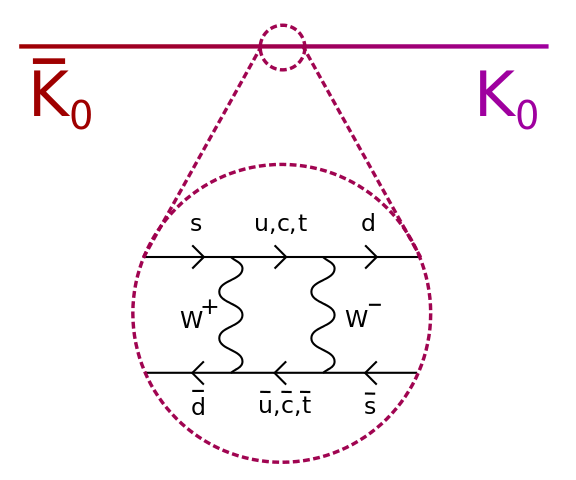
\includegraphics[width=0.4\linewidth]{img/Kaon-box-diagram-with-bar.svg.png}
    \end{center}
    \refimgsource{Wikimedia}{https://commons.wikimedia.org/wiki/File:Kaon-box-diagram-with-bar.svg}{24.01.2022}{Creative Commons Attribution-Share Alike 3.0 Unported}
\end{fquestion}

\begin{fquestion}{Wie wird dort die $CP$ Symmetrie gebrochen?}
    Unter der Parität $P$ und der Ladungskonjugation $C$ haben die beiden Kaonen die Abbildungsgleichung
    $$
    \begin{aligned}
        CP \ket{K^0} &= -\ket{\bar{K}^0}, &&& CP \ket{\bar{K}^0} &= -\ket{K^0}
    \end{aligned}
    $$
    Die Eigenzustände der $CP$ Operation sind entsprechend
    $$
    \begin{aligned}
        \ket{K_1^0} &= \frac{1}{\sqrt{2}} \left(\ket{K^0} - \ket{\bar{K}^0} \right), &&& \ket{K_2^0} &= \frac{1}{\sqrt{2}} \left(\ket{K^0} + \ket{\bar{K}^0} \right)
    \end{aligned}
    $$
    mit
    \(CP\ket{K_1^0} = + \ket{K_1^0}\) und \(CP\ket{K_2^0} = -\ket{K_2^0}\)
    Unter Annahme der $CP$ Erhaltung ergeben sich die beiden Zerfallskanäle $K_1^0 \rightarrow 2 \pi$ (schnell) und $K_2^0 \rightarrow 3\pi$ (langsam).
    In der Realität existieren ein langlebiger $K^0_L$ und ein kurzlebiger $K^0_S$ Kaonzustand, allerdings kann der langlebige ebenfalls in $2\pi$ zerfallen, weswegen dies keine $CP$ Eigenzustände sind und die Symmetrie entsprechend gebrochen ist.
\end{fquestion}

% \begin{question}{Wie sieht das bei Kaonen aus?}
%     Umwandlungsschema (Feynman-Diagramme), k und anti-K vs. $K_\text{short}$ und $K_\text{long}$
% \end{question}

\subsection{Laser}

\begin{fquestion}{Wie beschreibt man ein 2-Niveau System?}
    In einem 2-Niveau System gibt es drei Prozesse bei dem Übergang zwei Niveaus $N_1$ und $N_2$ ($E_1 < E_2$): Absorption $B_{12}$, sowie spontane $A_{21}$ und stimulierte $B_{21}$ Emission (mit den jeweiligen Einstein-Koeffizienten).
    Daraus ergibt sich die Ratengleichung
    $$\dot{N}_1 = -\dot{N}_2 = -B_{12} u N_1 + B_{21} u N_2 + A_{21} N_2$$
    in Abhängigkeit der spektralen Energiedichte $u$.
    Nach längerem Rechnen (mit der Boltzmann-Verteilung der Energieniveaus) erhält man $B_{12} = B_{21}$ (bei gleicher Entartung der Energieniveaus) und $A_{21} = \frac{8\pi h}{\lambda^3} B$.
    Außerdem erhält man im thermodynamischen Gleichgewicht 
    $$\frac{N_2}{N_1} = \frac{B_{12} u}{A_{21} + B_{21} u}$$
    was insbesondere mit den obigen Bedingungen bedeutet dass $N_2 < N_1$ und damit nie mehr Photonen stimuliert emittiert als absorbiert werden können.
\end{fquestion}

\begin{fquestion}{Wie funktioniert ein Laser?}
    Ein Laser funktioniert über die sogenannte \textit{Besetzungsinversion}. 
    Bei etwa einem 3- oder 4-Niveau-System kann es technisch erreicht werden, dass das Laserniveau $N_L$ höher bevölkert als der niedrigere Zustand ist.
\end{fquestion}

\begin{fquestion}{Wie sind die Übergänge bei einem 3-Niveau-Laser?}
    Bei einem 3-Niveau Laser gibt es drei Energieniveaus $E_1 < E_2 < E_3$. 
    Der Laser funktioniert dann über
    $$E_1 \xrightarrow{\text{Pumpen}} E_3 \xrightarrow[\text{Spontan}]{\text{Strahlungslos}} E_2 \xrightarrow{\textbf{Laserübergang}} E_1,$$
    wobei die Besetzungsinversion zwischen $E_1$ und $E_2$ stattfindet.
    Dafür muss der Zustand $E_2$ im Vergleich zum Zustand $E_3$ eine relativ große Lebensdauer haben.
    
    Ein typischer Vertreter ist der Rubinlaser.
\end{fquestion}

\begin{fquestion}{Wie sind die Übergänge bei einem 4-Niveau-Laser?}
    Bei einem 4-Niveau Laser gibt es drei Energieniveaus $E_1 < E_2 < E_3 < E_4$. 
    Der Laser funktioniert dann über
    $$E_1 \xrightarrow{\text{Pumpen}} E_4 \xrightarrow[\text{Spontan}]{\text{Strahlungslos}} E_3 \xrightarrow{\textbf{Laserübergang}} E_2 \xrightarrow{\text{Schnell}} E_1,$$
    wobei die Besetzungsinversion zwischen $E_2$ und $E_3$ stattfindet, da sich $E_2$ schnell wieder in den Grundzustand abgeregt und damit quasi nicht besetzt ist.
    Dadurch ist für die Besetzungsinversion weniger Energie erforderlich (höheres Inversionsverhältnis).
    
    Typische Vertreter sind der Diodenlaser, der Farbstofflaser und der Helium-Neon-Laser.
\end{fquestion}

% \begin{question}{Was ist die Grundbedingung für einen Laser?}
%     Besetzungsinversion
% \end{question}

% \begin{question}{Wo ist der Laserübergang bei einem 4-Niveau Laser?}
%     Zwischen $E_3$ und $E_2$, also den zwei Niveaus, die eine kleinere Energiedifferenz aufweisen.
% \end{question}

% \begin{fquestion}{Welche Zustände müssen kurzlebig sein, welche müssen langlebig sein?}
%     Der Grundzustand $E_1$ und der angeregte Zustand $E_3$ müssen langlebig sein ($E_3$ heißt auch metastabil), die anderen beiden kurzlebig.
%     Die Besetzungsinversion erfolgt dann über 
%     $$E_1 \overset{\mathrm{Pumpen}}{\longrightarrow} E_4 \overset{\mathrm{strahlungslos} }{\longrightarrow} E_3.$$
% \end{fquestion}

\begin{fquestion}{Wie erreicht man langlebige Niveaus?}
    Langlebige oder metastabile Niveaus erreicht man durch dadurch, dass eine Auswahlregel die zum Übergang führt verboten ist und dadurch der Übergang unterdrückt wird.
    
    Besonders effektiv ist die Unterdrückung des $l=1$ Dipolübergangs, da die Übergangswahrscheinlichkeit $P \propto E_\gamma^{2j + 1}$ ist und entsprechend klein für große Momente.
\end{fquestion}

% \begin{question}{Was heißt langlebig, wie realisiert man das?}
%     Falls beispielsweise ein elektrischer Dipolübergang erlaubt ist, ist ein Zustand meist kurzlebig.
%     Umgekehrt ist ein Zustand langlebig, falls ein solcher $E_1$-Übergang nicht erlaubt ist (siehe Multipolstrahlung).
% \end{question}

% \begin{question}{Was sind Unterschiede zwischen 3- und 4-Niveau-Lasern?}
%     Beim 3-Niveau-Laser erfolgt der ``lasende'' Übergang zwischen $E_2$ und dem Grundzustand $E_1$.
%     Für die Besetzungsinversion muss also mehr als die Hälfte der Elektronen in die angeregten Zustände befördert werden, was viel Energie benötigt.
%     Beim 4-Niveau-Laser ist der Übergang von $E_3$ zu $E_2$.
%     Da $E_2$ kurzlebig ist, kann dieses Niveau quasi als leer betrachtet werden.
%     Für die Besetzungsinversion ist also weniger Energie erforderlich.
%     % \\
%     % Ein 3-Niveau-Laser hat einen gepulsten Output, ein 4-Niveau-Laser einen kontinuierlichen ???
% \end{question}

% \begin{question}{Wie sieht die Lebensdauer aus?}
%     Übergangswahrscheinlichkeit ist proportional zu $E^{(2j+1)}$ ??? 
%     verbotene/erlaubte übergänge ??? 
%     Spontane Emission: $10^8 1/s$
% \end{question}

\begin{fquestion}{Kann es auch Laser im Röntgenbereich geben?}
    Nein, klassisch nicht weil der Einstein-Koeffizient der spontanen Emission $A \propto \nu^3$, entsprechend dominiert bei großen $\nu$ die spontane Emission (Anmerkung: es sind Laser im niedrigen Röntgenbereich realisiert worden, z.B. $\SI{2.7}{nm}$ von Chang et. al. in 1997).
    
    Man kann aber über beispielsweise Synchrotron-Strahlung Strahlungsquellen im Röntgenbereich konstruieren.
\end{fquestion}
